\documentclass{beamer}
\usepackage{graphicx}

\title{Verified Metatheory and Type Inference for a Name-Carrying Simply-Typed $\lambda$-Calculus}
\author{Michael Rawson}
\date{Lent Term 2017}

\begin{document}
\frame{\titlepage}

\begin{frame}
\frametitle{Simply-Typed $\lambda$-Calculus}
\begin{align*}
M &::= x\ |\ \lambda \alert{(x : T)}.M\ |\ (M\ M)\\
T &::= T_0\ |\ T_1\ |\ \ldots\ |\ T \to T
\end{align*}

\begin{itemize}
\item $\lambda$-calculus, plus a na\"ive typing system
\item terms are familiar $\lambda$-terms, plus a \alert{typing annotation}
\item types are either a base type $T_n$ or a function type
\end{itemize}
\end{frame}

\begin{frame}
\frametitle{Names and $\alpha$-Equivalence}
Suppose
$$
f(x) = M(x)
$$
and
$$
g(y) = M(y)
$$

\begin{itemize}
\item Reasonably conclude $f = g$, though they differ in variable names
\item Would like to have $\lambda x.x = \lambda y.y$
\item Unusual approach to this problem: ``can I swap variable names to make them equal?''
\end{itemize}
\end{frame}

\begin{frame}
\frametitle{Verification with Isabelle}
\begin{center}
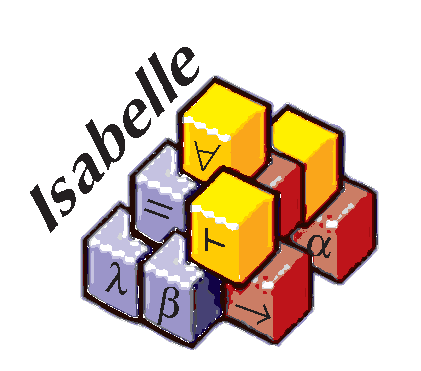
\includegraphics[width=0.3\textwidth]{logo}
\end{center}
\begin{itemize}
\item machine-checked mathematical proof
\item arguments \emph{cannot} contain logical errors
\item ...but quite tricky to argue rigorously enough!
\item tooling to make this easier
\end{itemize}
\end{frame}

\begin{frame}
\frametitle{Progress}
\begin{center}
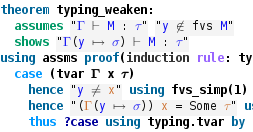
\includegraphics[width=0.5\textwidth]{screenshot}
\end{center}

\begin{itemize}
\item Terms \emph{quotiented} with respect to $\alpha$-equivalence
\item Typing and evaluation relations on these terms
\item Metatheory: \emph{progress}, \emph{preservation}
\item Verified type-inference algorithm
\item Currrently refactoring and adding more metatheory
\end{itemize}
\end{frame}

\begin{frame}
\frametitle{Finish}
\end{frame}
\end{document}
